\documentclass[10pt]{beamer}

%STANDARD PREAMBLE
%https://tex.stackexchange.com/questions/68821/is-it-possible-to-create-a-latex-preamble-header
\usepackage{/Users/mwojno01/Repos/latex_preamble/beamer_preamble}

% DOCUMENT SPECIFIC STUFF
% using default arg uments; see https://stackoverflow.com/questions/1812214/latex-optional-arguments

%%% 
% SPECIFIC TO THIS DOCUMENT
%%%

% FASTER LIMITS, INTEGRALS AND SUMS
\newcommand{\dlim}{\ds\lim}
\newcommand{\dint}{\ds\int}
\newcommand{\dsum}{\ds\sum}
\newcommand{\dmu}{\wrt{\mu}}

% SIGMA-FIELDS 
% Sigma fields (text)
\renewcommand{\sf}{$\sigma$-field}
\newcommand{\sfs}{$\sigma$-fields}


% CARATHEODORY
\newcommand{\Caratheodory}{Carath\'eodory}


%%%% Citations should be rendered differently in beamer -- ADD TO BEAMER

\title{Constructing measures}
\subtitle{...on spaces with unit, finite, and infinite dimensionality}

\begin{document}

\maketitle


\begin{frame}[standout]
Goal: Construct \alert{measures} on interesting spaces
\end{frame}

\begin{frame}{Table of contents}
  \setbeamertemplate{section in toc}[sections numbered]
  \tableofcontents[hideallsubsections]
\end{frame}

\section{Background}
\begin{frame}{Measures are defined on \alert{\sfs}}
\begin{definition}
Let $\F$ be a collection of subsets of a set $\Omega$.  Then $\F$ is called a \textbf{sigma-field}  if it satisfies

\begin{enumerate}
	\item $\Omega \in \F$ 
	\item \textit{(Closed under complementation.)} If $A \in \F$, then $A^c \in \F$.
	\item \textit{(Closed under countable unions.)} If $A_1,A_2, ... \in \F$ then $\cup_{i=1}^\infty A_i \in \F$.  
\end{enumerate}
\end{definition}

%\begin{remark}
%It follows that $\sigma$-fields are closed under countable intersections, since
%\[ \cap_{i=1}^\infty A_i \stackrel{\text{DeMorgan's Law}}{=} (\cup_{i=1}^\infty A_i^c)^c \]	
%\end{remark}

%\pause 
%\begin{block}{Example}
%$\F =\set{\emptyset, \Omega}$ is the smallest \sf\ on $\Omega$. 
%\end{block}
%
%\pause 
%\begin{block}{Example}
%	$\F =2^\Omega$, i.e. the set of all subsets of $\Omega$, is the largest \sf\ on $\Omega$.
%\end{block}
\pause
\begin{block}{Remark}
The definition implies that sigma-field are also closed under countable \textit{intersections}.	
\end{block}

\pause 
\begin{block}{Example}
If $A \in \Omega$ is non-empty, then $\F = \set{\emptyset, A, A^c, \Omega}$ is the smallest \sf\ containing $A$.
\end{block}


%\pause 
%\begin{block}{Definition}
%$\F$ is called a \textbf{field} if 
%	
%\end{block}

\pause 
\begin{block}{Definitions}
A set $A \in \F$ is called a \textbf{measurable set}.\\
$(\Omega, \F)$ is called a \textbf{measurable space}.	
\end{block}


\end{frame}

\begin{frame}{Measures}	
\begin{definition}
A \textbf{measure} on a \sf~$\F$ is a non-negative, extended real-valued function $\mu$ on $\F$ such that whenever $A_1, A_2, ...$ form a finite or countably infinite collection of disjoint sets in $\F$, we have \alert{countable additivity}; that is,
\[ \mu \bigg( \bigcupdot_n A_n \bigg) = \ds\sum_n \mu(A_n) \]
\label{def:measure}	
\end{definition}

\pause 
\begin{block}{Example}
A \textbf{probability measure} is a measure where $\mu(\Omega)=1$.		
\end{block}
\end{frame}

\section{One dimension: Lebesgue measure}

\begin{frame}{Elementary Families}

\begin{definition}
An \textbf{elementary family} is a collection $\scriptE$ of subsets of $\Omega$ such that 
\begin{enumerate}
\item $\emptyset \in \scriptE$
\item if $E,F \in \scriptE$ then $\scriptE \cap \F \in \scriptE$
\item if $E \in \scriptE$, then $E^c$ is a finite disjoint union of members of $\scriptE$.	
\end{enumerate}
\label{def:elementary_family}
\end{definition}

\begin{block}{Example}
Consider the \textbf{right semi-closed (r.s.c) intervals}:
\centering
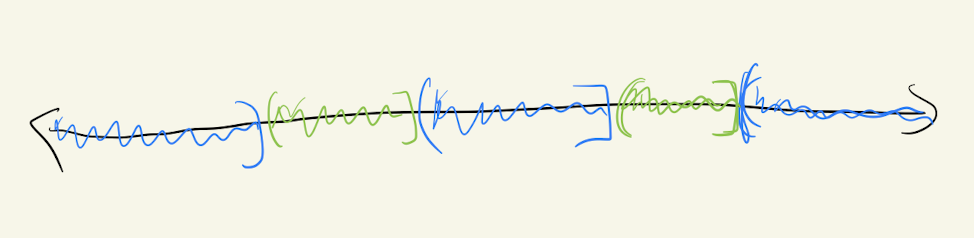
\includegraphics[width=.8\textwidth]{images/rsc_intervals}
\end{block}	
\end{frame}



\begin{frame}{From elementary families to fields}

\begin{definition}
Let $\F_0$ be a collection of subsets of a set $\Omega$.  Then $\F_0$ is called a \textbf{field}  if it satisfies

\begin{enumerate}
	\item $\Omega \in \F_0$ 
	\item \textit{(Closed under complementation.)} If $A \in \F_0$, then $A^c \in \F_0$.
	\item \textit{(Closed under \alert{finite} unions.)} If $A_1,A_2, ... \in \F_0$ then $\cup_{i=1}^n A_i \in \F_0$.  
\end{enumerate}
\end{definition}

\pause 
\begin{proposition}
If $\scriptE$ is an elementary family then the collection 
\[ \F_0 := \set{ \text{finite disjoint unions of members of } \scriptE} \]
is a field.
\label{prop:from_elementary_families_to_fields}	
\end{proposition}


\pause 
\begin{block}{Example}
The collection of \textbf{finite disjoint unions of r.s.c intervals} forms a field:
\centering
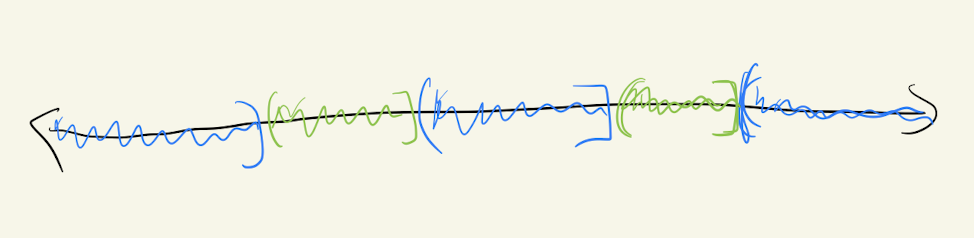
\includegraphics[width=.6\textwidth]{images/rsc_intervals}
\end{block}	
\end{frame}


\begin{frame}{Pre-measure on a field}
\begin{block}{Example: Lebesgue pre-measure}
To measure a finite disjoint union of r.s.c intervals
\begin{figure}
\centering
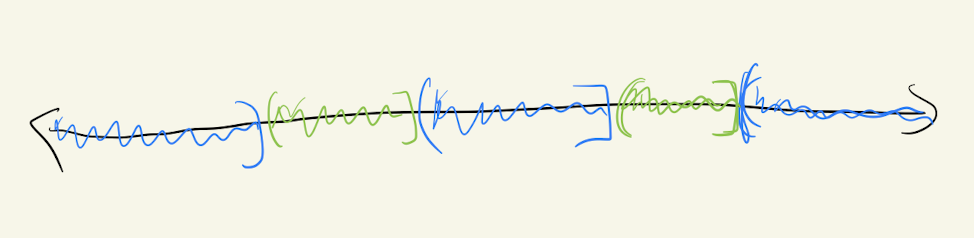
\includegraphics[width=.8\textwidth]{images/rsc_intervals}
\end{figure}
Set
\begin{align*}
%	\mu(a,b]& = b-a \\
	\mu \bigg(\bigcupdot_{i=1}^n (a_i, b_i] \bigg) &= \ds\sum_{i=1}^n b_i - a_i 
\end{align*}
%This is \textit{Lebesgue pre-measure} (i.e., Lebesgue measure on a field).
\end{block}



\end{frame}

\begin{frame}{\Caratheodory~Extension Theorem}
\begin{theorem} Let $\mu$ be a pre-measure on a field $\F_0$ of subsets of $\Omega$, and assume that $\mu$ is $\sigma$-finite on $\F_0$.  Then $\mu$ has a unique extension to a measure on $\F := \sigma(\F_0)$, the minimal $\sigma$-field over $\F_0$. 
 \label{thm:caratheodory_extension}
\end{theorem}

\begin{block}{Now we can measure all sorts of things:}
\begin{align*}
	[a,b] &= \bigcap_{n=1}^\infty \bigg(a-\frac{1}{n}, b\bigg] && \tinytext{Closed intervals} \\
	(a,b) &= \bigcup_{n=1}^\infty \bigg(a, b-\frac{1}{n}\bigg] && \tinytext{Open intervals} \\
	\texttt{Cantor set} &= \bigcap_{i=1}^\infty\bigcap_{j=1}^{3^{i-1}-1}\left[0,\frac{3j+1}{3^i}\right]\cup \left[\frac{3j+2}{3^i}, 1\right]&& \tinytext{Weird things} \\
	\\
	\vdots & \quad \quad  \vdots && \vdots \\
\end{align*}

\end{block}
	
\end{frame}




\section{$n$ dimensions: Product measure}

\begin{frame}{Measurable rectangles}

Let $(X,\M)$ and $(Y,\N)$ be measurable spaces (i.e. sets and associated \sfs).

\begin{definition}
 A \textbf{measurable rectangle} is a subset $A \times B$ of $X \times Y$ where $A \in \M$ and $B \in \N$ are measurable subsets of $X$ and $Y$, respectively.
\end{definition}
%
%\begin{remark}{\remarktitle{Measurable rectangles need not have intervals for ``sides".}}
%The ``sides" of a measurable rectangle $A \times B$ are not required to be intervals.  For instance, if $\R$ is equipped with the Borel $\sigma$-field, then $\Q \times \Q$ is a measurable rectangle in $\R \times \R$. 	
%\end{remark}

\begin{block}{Examples}
 \begin{tabular}{cl}
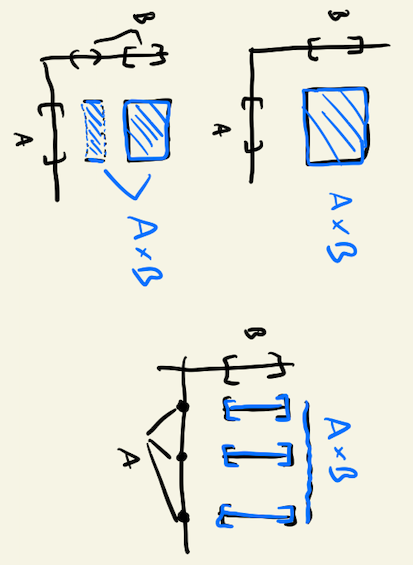
\includegraphics[width=.4\textwidth, angle=90]{images/measurable_rectangles}	&
 \parbox[b]{0.4\linewidth}{Note: The ``sides" of a measurable rectangle $A \times B$ are not required to be intervals.  For instance, if $\R$ is equipped with the Borel $\sigma$-field, then $\mathbb{Q} \times \mathbb{Q}$ is a measurable rectangle in $\R \times \R$.}
\end{tabular}

\end{block}

\end{frame}


\begin{frame}{Measurable rectangles are an elementary family.}
For example, measurable rectangles are closed under intersection.
\begin{figure}[H]
\centering 
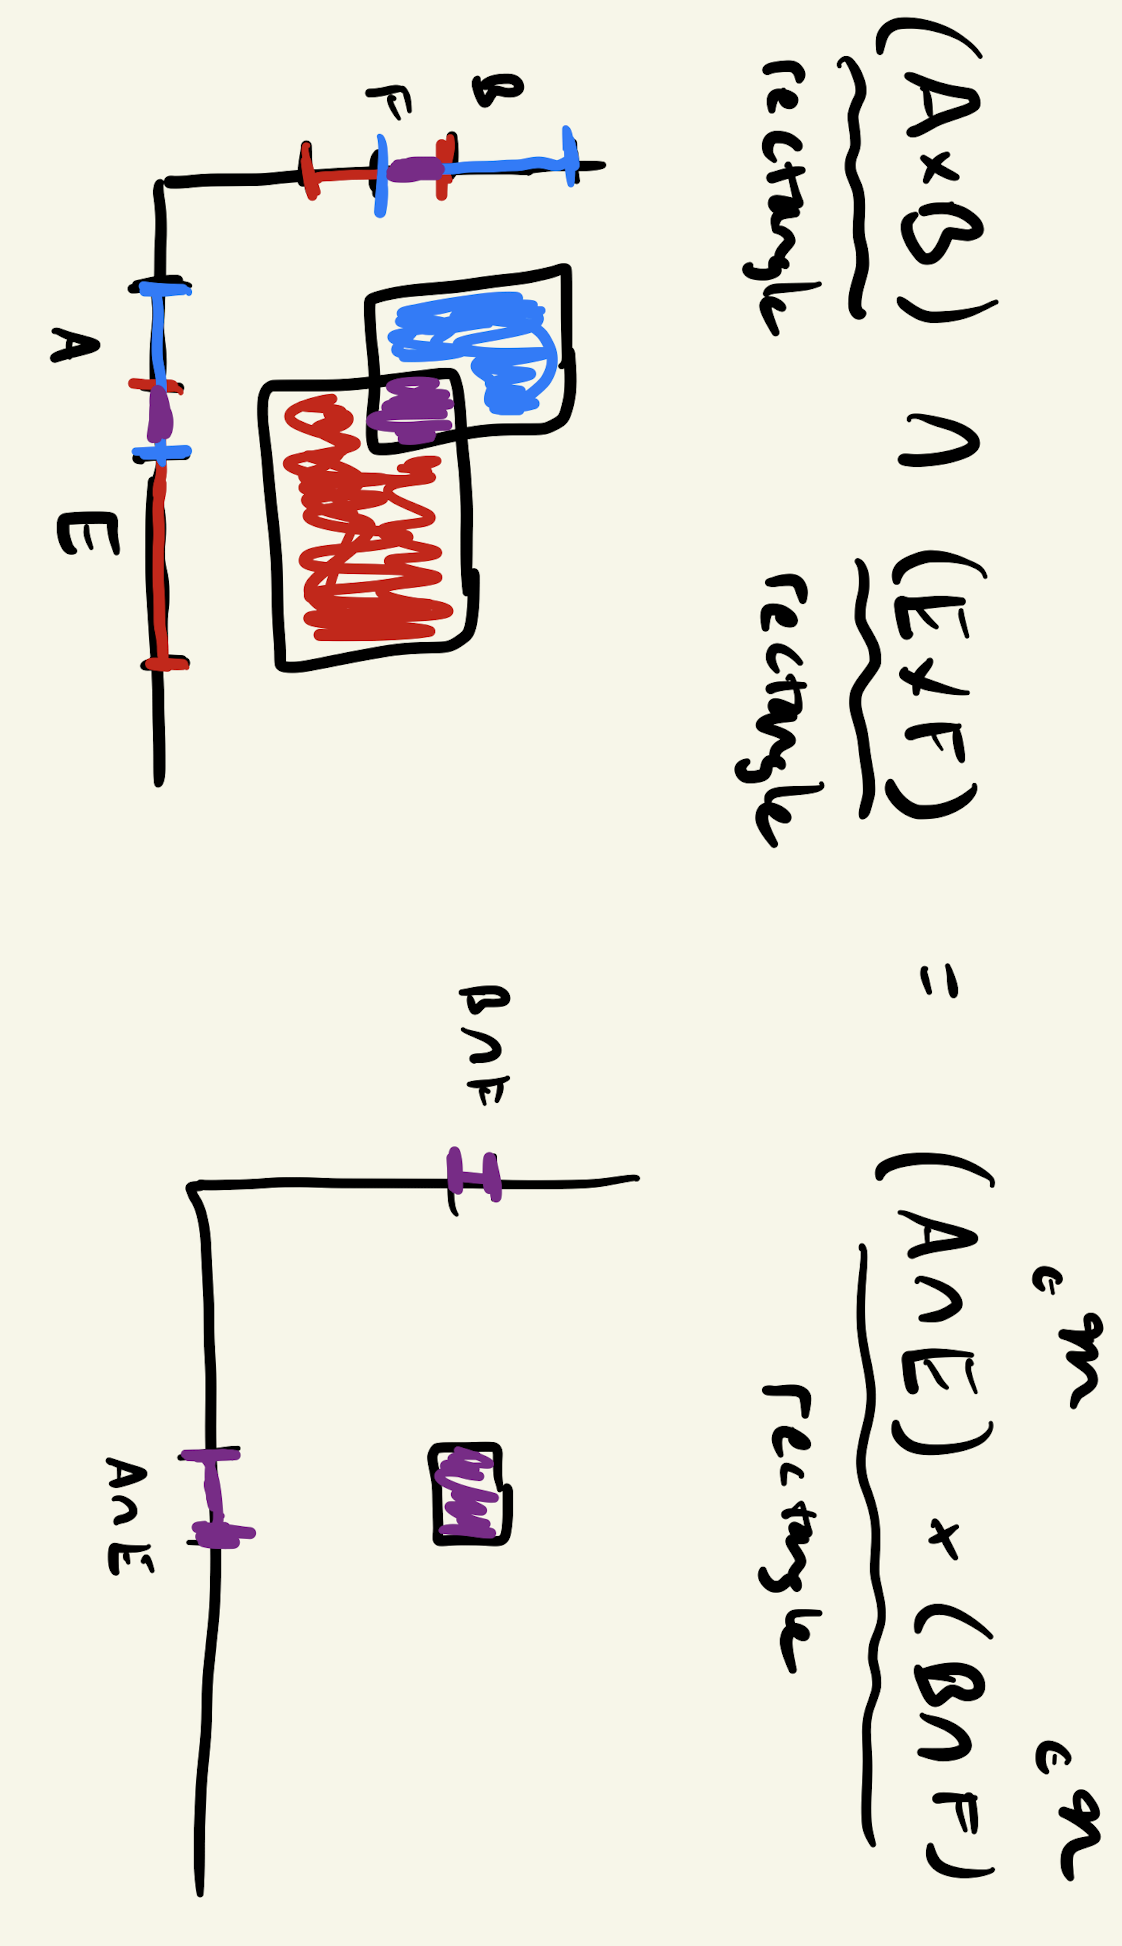
\includegraphics[width=.4\textwidth, angle=90]{images/rectangles_are_closed_under_intersection}
\end{figure}
\end{frame}

\begin{frame}{Construction of the product measure}
Let $(X,\M, \mu)$ and $(Y,\N, \nu)$ be measure spaces.

Let $C \in F_0$ be a finite disjoint union of rectangles $A_1 \times B_1, A_2 \times B_2, \hdots A_n \times B_n$. 

Define the set function 
\[ \pi_0 (C) := \ds\sum_{i=1}^n \mu(A_i) \nu(B_i) \]
Then $\pi_0$ is well-defined, and a premeasure on $\F_0$.

By the \Caratheodory~Extension Theorem, $\pi_0$ extends to a measure $\pi$ on $\F:=\sigma(\F_0)$.	
\end{frame}

\begin{frame}{Application}

To find the product measure of $D$, an arbitrary measurable set in $X \times Y = \R^2$

\begin{figure}[H]
\centering 
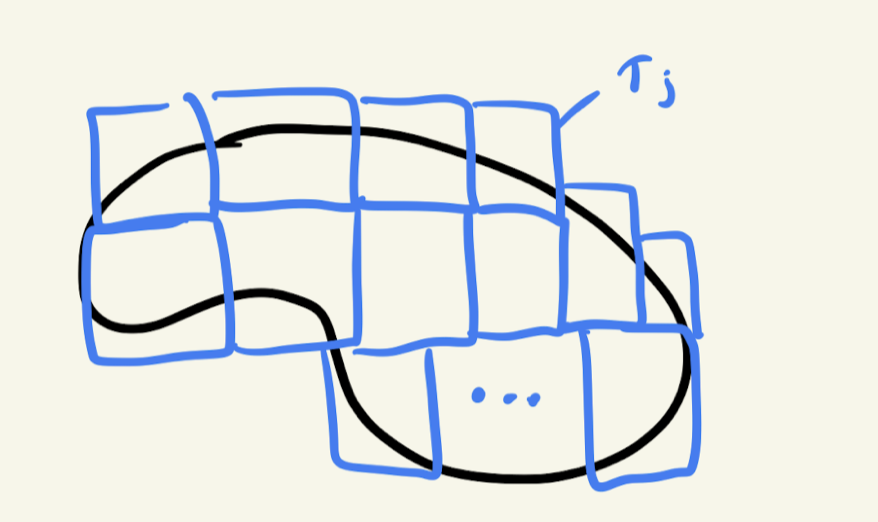
\includegraphics[width=.4\textwidth]{images/measuring_a_set_in_2dim}
\end{figure}


We take the least upper bound of the measure of countable rectangles which cover it. 
\begin{align}
\mu \times \nu(D): = \inf \bigg\{ \ds\sum_{n=1}^\infty \mu(A_n) \nu(B_n) : \cup_{n=1}^\infty (A_n \times B_n) \supseteq D, \; A_n, B_n \in \B(\R)\bigg\} 
\end{align}	
\end{frame}


\section{Infinite dimensions}

\begin{frame}{Measurable cylinders -- an elementary family}
\begin{tabular}{cc}
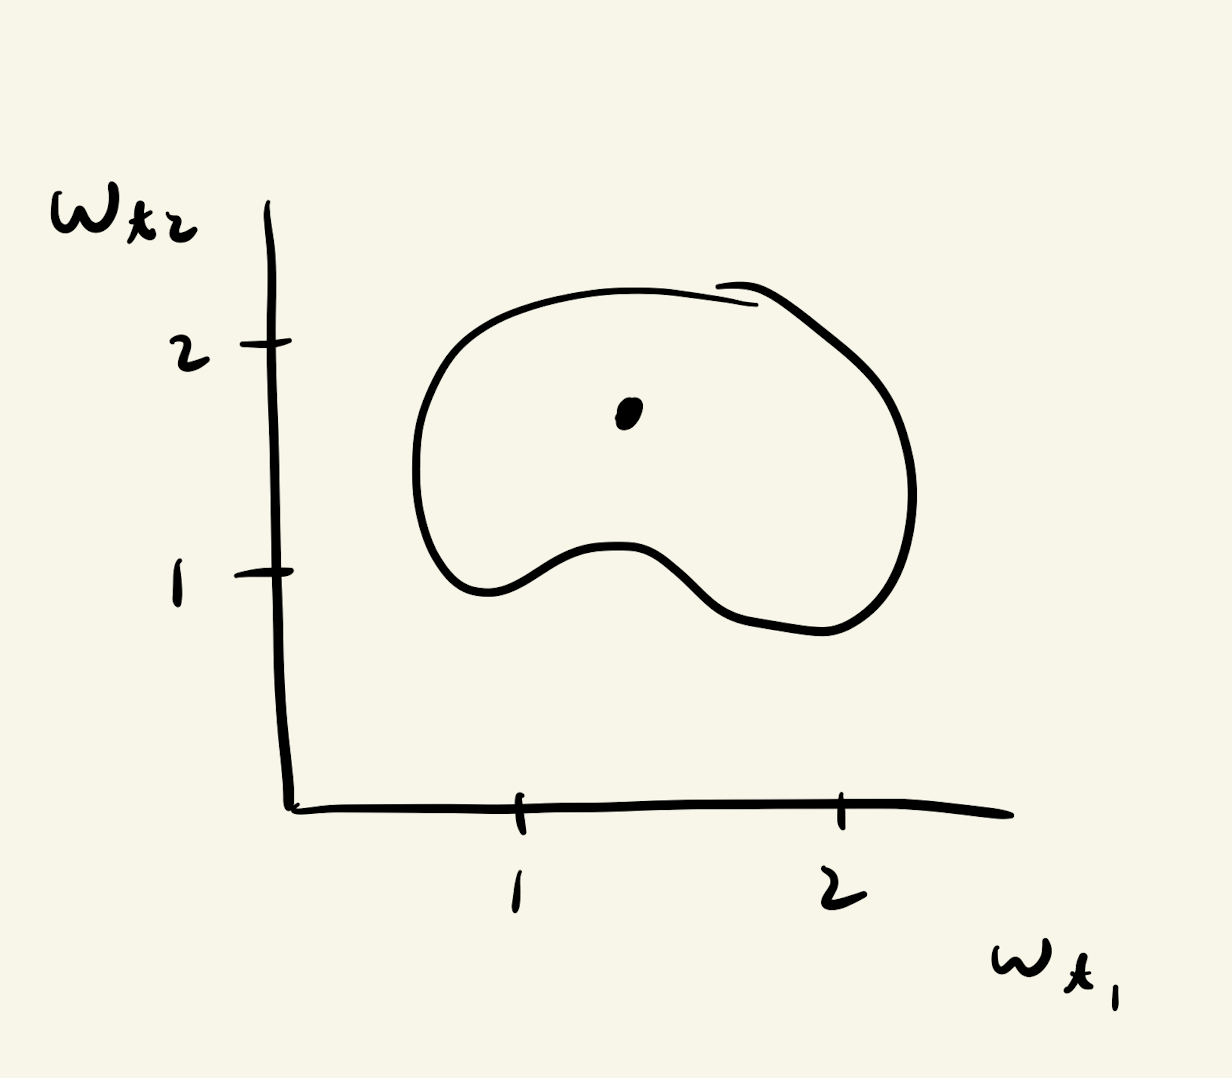
\includegraphics[width=.4\textwidth]{images/cylinder_base_in_2_coordinates} &
  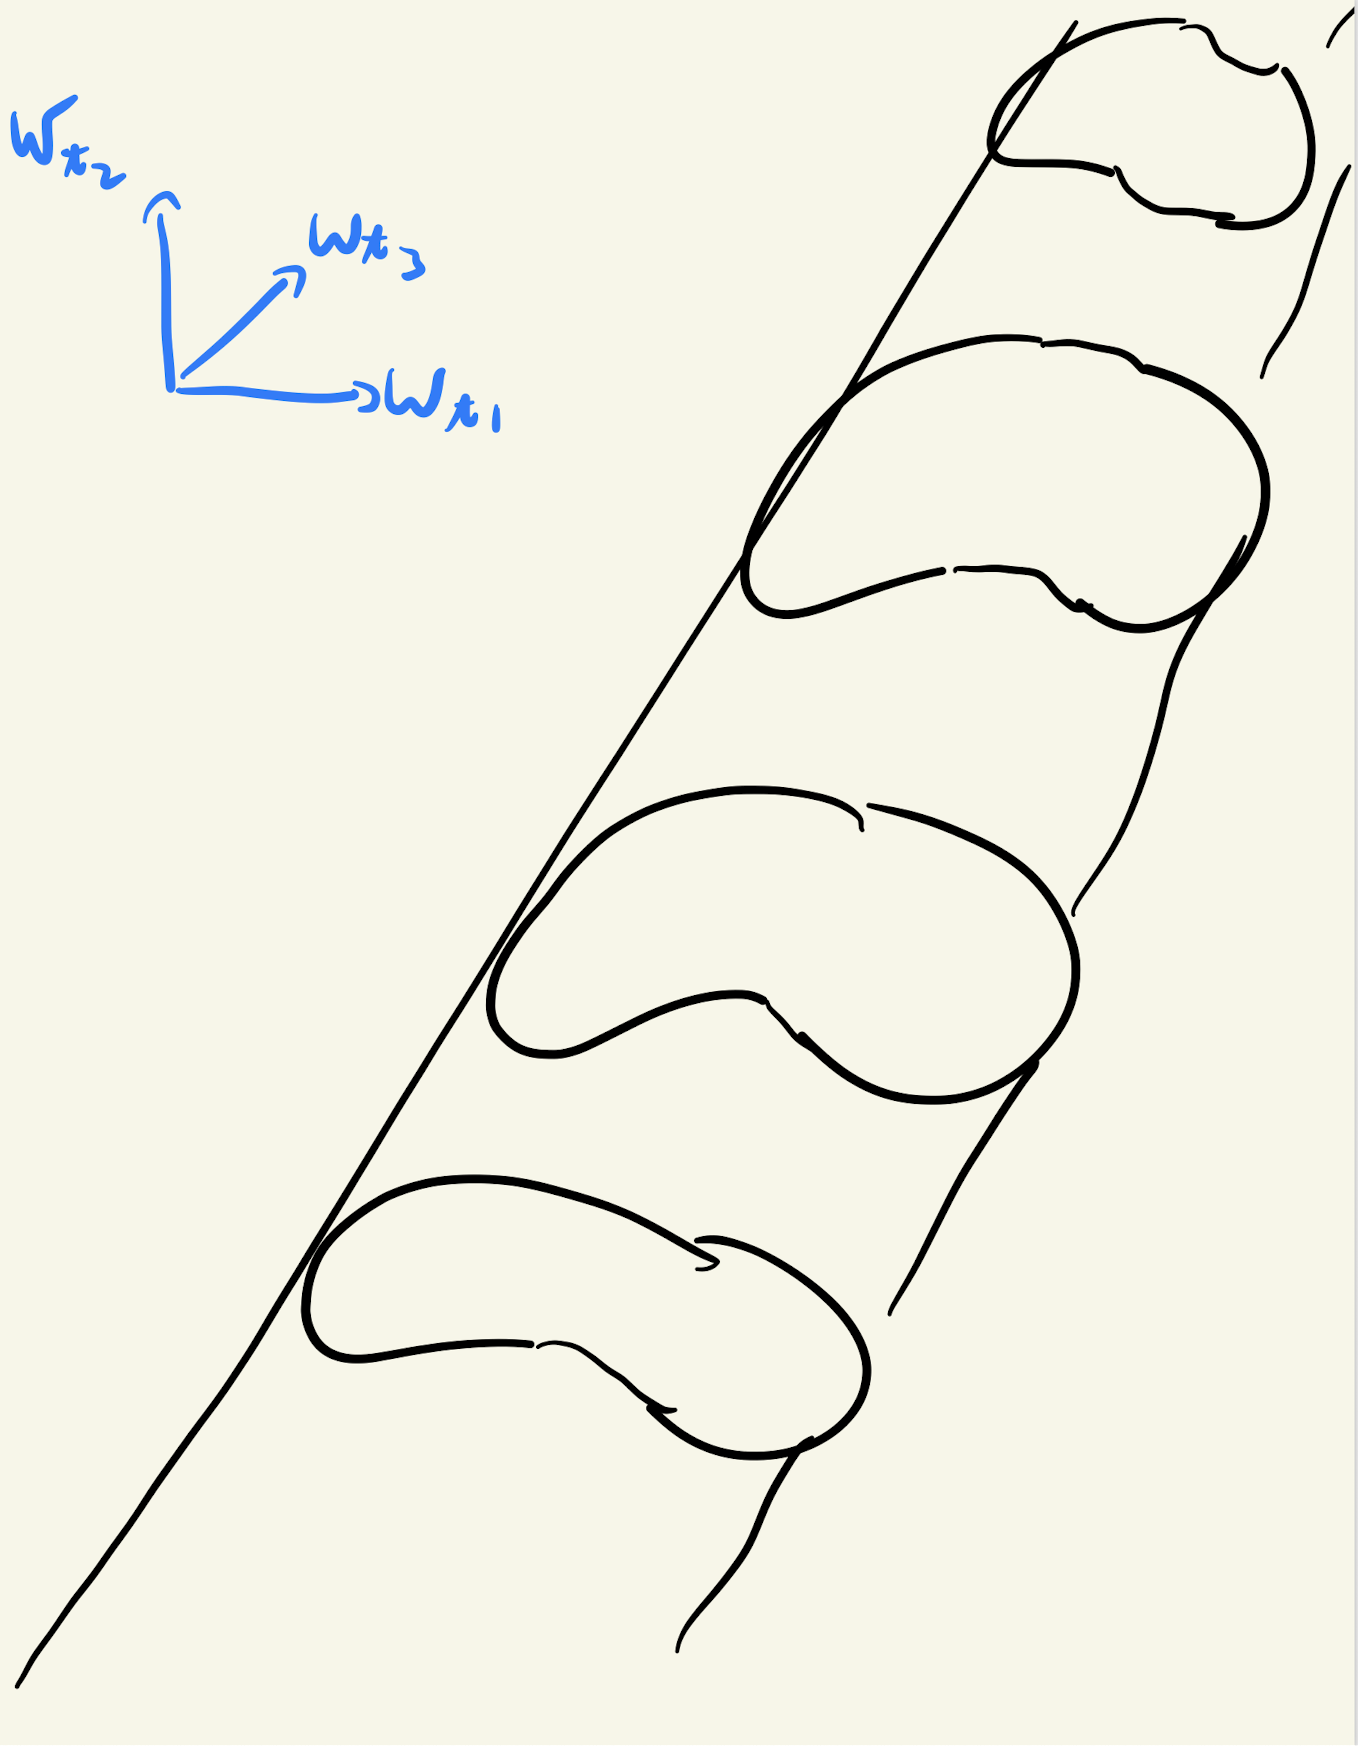
\includegraphics[width=.4\textwidth]{images/cylinder_projected_to_first_three_coordinates} \\
  \parbox[b]{0.4\linewidth}{A base (in 2 coordinates) for a cylinder} &  \parbox[b]{0.4\linewidth}{The cylinder projected to the first three coordinates.}
\end{tabular}
\end{frame}

\end{document}



